\documentclass{exam}
\usepackage{../../commonheader}
\lstset{language=Scheme}
%%% CHANGE THESE %%%%%%%%%%%%%%%%%%%%%%%%%%%%%%%%%%%%%%%%%%%%%%%%%%%%%%%%%%%%%%
\discnumber{6}
\title{\textsc{Scheme}}
\date{March 20 to March 24, 2017}
%%%%%%%%%%%%%%%%%%%%%%%%%%%%%%%%%%%%%%%%%%%%%%%%%%%%%%%%%%%%%%%%%%%%%%%%%%%%%%%

\begin{document}
\maketitle
\rule{\textwidth}{0.15em}
\fontsize{12}{15}\selectfont

%%% INCLUDE TOPICS HERE %%%%%%%%%%%%%%%%%%%%%%%%%%%%%%%%%%%%%%%%%%%%%%%%%%%%%%%


%%% Question %%%

\begin{blocksection}
Scheme is a programming language, much like Python. In fact, many of Python's design features were inspired by Scheme. The point of learning this language is twofold: one, we're looking into what parts of Python generalize to other languages. Two, we want to start thinking about how to design and build (an interpreter  for) a programming language, and it turns out Scheme is a nice one to build. In fact, we'll show you enough of the language in this hour to write recursive procedures. This section covers the basics. You'll learn the rest in lab and discussion. It's pretty awesome that we'll be picking up a whole new programming language within an hour.
\newline
\newline
\textbf{Useful Resources:}
\begin{itemize}
    \item CS61A Online Scheme Interpreter: \texttt{scheme.cs61a.org}
    \begin{itemize}
        \item To see the box and pointer diagrams for lists, do \texttt{(demo `autopair)}
    \end{itemize}
\end{itemize}
\end{blocksection}

\section{What Would Scheme Print?}
\begin{questions}
\begin{blocksection}
\question What will Scheme output? Draw box-and-pointer diagrams to help determine this.

\begin{lstlisting}
scm> 3.14
\end{lstlisting}
\begin{solution}[0.25in] 
\texttt{3.14}
\end{solution}

\begin{lstlisting}
scm> pi
\end{lstlisting}
\begin{solution}[0.25in]
\texttt{Error}
\end{solution}

\begin{lstlisting}
scm> (define pi 3.14)
\end{lstlisting}
\begin{solution}[0.25in]
\texttt{pi}
\end{solution}

\begin{lstlisting}
scm> pi
\end{lstlisting}
\begin{solution}[.25in]
\texttt{3.14}
\end{solution}

\begin{lstlisting}
scm> 'pi
\end{lstlisting}
\begin{solution}[.25in]
\texttt{pi}
\end{solution}

\begin{lstlisting}
scm> (if 2 3 4)
\end{lstlisting}
\begin{solution}[.25in]
\texttt{3}
\end{solution}

\begin{lstlisting}
scm> (if 0 3 4)
\end{lstlisting}
\begin{solution}[.25in]
\texttt{3}
\end{solution}

\begin{lstlisting}
scm> (if #f 3 4)
\end{lstlisting}
\begin{solution}[.25in]
\texttt{4}
\end{solution}

\begin{lstlisting}
scm> (if nil 3 4)
\end{lstlisting}
\begin{solution}[.25in]
\texttt{3}
\end{solution}

\begin{lstlisting}
scm> (if (= 1 1) 'hello 'goodbye)
\end{lstlisting}
\begin{solution}[.25in]
\texttt{hello}
\end{solution}
\end{blocksection}

\begin{blocksection}
\begin{lstlisting}
scm> (define (factorial n)
        (if (= n 0)
            1
            (* n (factorial (- n 1)) )))
\end{lstlisting}
\begin{solution}[.25in]
\texttt{factorial}
\end{solution}

\begin{lstlisting}
scm> (factorial 5)
\end{lstlisting}
\begin{solution}[.25in]
\texttt{120}
\end{solution}

\begin{lstlisting}
scm> (= 2 3)
\end{lstlisting}
\begin{solution}[.25in]
\texttt{\#f}
\end{solution}

\begin{lstlisting}
scm> (= '() '())
\end{lstlisting}
\begin{solution}[.25in]
\texttt{Error}
\end{solution}

\begin{lstlisting}
scm> (eq? '() '())
\end{lstlisting}
\begin{solution}[.25in]
\texttt{\#t}
\end{solution}

\begin{lstlisting}
scm> (eq? nil nil)
\end{lstlisting}
\begin{solution}[.25in]
\texttt{\#t}
\end{solution}

\begin{lstlisting}
scm> (eq? '() nil)
\end{lstlisting}
\begin{solution}[.25in]
\texttt{\#t}
\end{solution}

\begin{lstlisting}
scm> (pair? (cons 1 2))
\end{lstlisting}
\begin{solution}[.25in]
\texttt{\#t}
\end{solution}

\begin{lstlisting}
scm> (list? (cons 1 2))
\end{lstlisting}
\begin{solution}[.25in]
\texttt{\#f}
\end{solution}
\end{blocksection}

\section{Code Writing in Scheme}

%%% Question %%%
\begin{blocksection}
\question \textbf{Hailstone once again!} Define a program called \texttt{hailstone}, which takes in two numbers \texttt{seed} and \texttt{n}, and returns the \texttt{n}th hailstone number in the sequence starting at seed. Assume the hailstone sequence starting at seed is longer or equal to n. As a reminder, to get the next number in the sequence, if the number is even, divide by two. Else, multiply by 3 and add 1. \newline

\textbf{Useful procedures to know:} \newline
\begin{enumerate}
\item \texttt{quotient}: floor divides, much like // in python
\subitem \texttt{(quotient 103 10)} outputs 10
\item \texttt{remainder}: takes two numbers and computes the remainder of dividing the first number by the second
\subitem \texttt{(remainder 103 10)} outputs 3
\end{enumerate}

\begin{nonsol}
\begin{lstlisting}
; The hailstone sequence starting at seed = 10 would be
; 10 => 5 => 16 => 8 => 4 => 2 => 1

; Doctests
> (hailstone 10 0)
10
> (hailstone 10 1)
5
> (hailstone 10 2)
16
> (hailstone 5 1)
16
> (hailstone 5 5)
1
\end{lstlisting}
\end{nonsol}

\begin{solution}[1in]
\begin{lstlisting}
(define (hailstone seed n)
    (if (= n 0)
        seed
        (if (= 0 (remainder seed 2))
            (hailstone
            (quotient seed 2)
            (- n 1)
           )
          (hailstone
          (+ 1 (* seed 3))
          (- n 1)
         )
    )
)
\end{lstlisting}
\end{solution}
\end{blocksection}

%%% Question %%%
\section{Scheme Lists}
\begin{blocksection}
\begin{nonsol}
Scheme has linked lists built in. You can make the following analogy:
\begin{center}
\begin{tabular}{ |l|l| }
\hline
 \texttt{Link(1, Link.empty)} & \texttt{(cons 1 nil)} \\
 \texttt{a = Link(1, Link(2, Link.empty))} & \texttt{(define a (cons 1 (cons 2 nil)))}  \\
 \texttt{a.first} & \texttt{(car a)} \\
 \texttt{a.rest} & \texttt{(cdr a)} \\
 \hline
\end{tabular}
\end{center}
However, \textbf{Scheme \texttt{cons} is more powerful}, as it allows its second argument to not be a list. Try the following out in the interpreter. Draw box and pointers when appropriate. Ask your mentor if you're unsure what's going on. You aren't expected to understand this completely on your own.
\question What will Scheme output? Draw box-and-pointer diagrams to help determine this.
\end{nonsol}

\begin{lstlisting}
scm> (cons 1 2)
\end{lstlisting}
\begin{solution}[0.25in]
\texttt{(1 . 2)}
\begin{center}
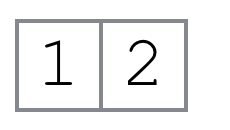
\includegraphics[scale=1]{scheme_lists_1}
\end{center}
\end{solution}

\begin{lstlisting}
scm> (cons 1 (cons 2 nil))
\end{lstlisting}
\begin{solution}[0.25in]
\texttt{(1 2)}
\begin{center}

\includegraphics[scale=0.7]{scheme_lists_2}
\end{center}
\end{solution}

\begin{lstlisting}
scm> (cons 1 '(2 3 4 5))
\end{lstlisting}
\begin{solution}[0.25in]
\texttt{(1 2 3 4 5)}
\begin{center}
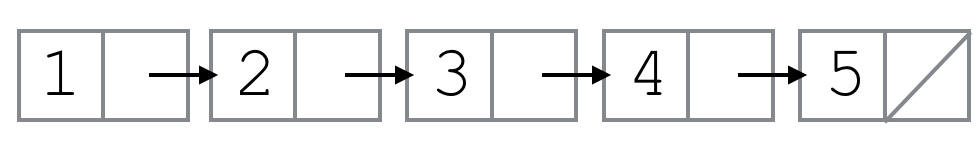
\includegraphics[scale=0.7]{scheme_lists_3}
\end{center}
\end{solution}

\begin{lstlisting}
scm> (cons 1 '(2 (cons 3 4))
\end{lstlisting}
\begin{solution}[0.25in]
\texttt{(1 2 (cons 3 4))}
\begin{center}
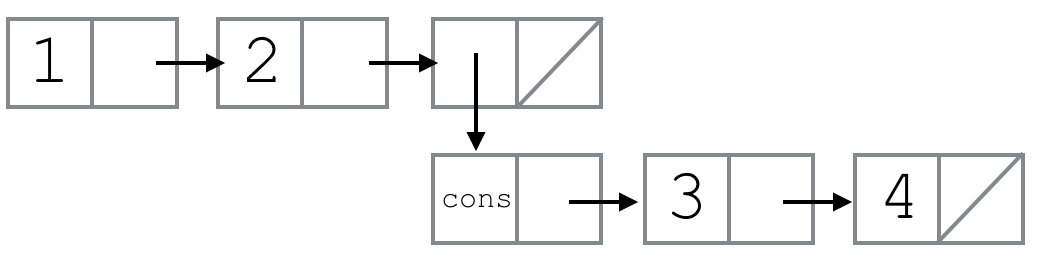
\includegraphics[scale=0.7]{scheme_lists_4}
\end{center}
\end{solution}

\begin{lstlisting}
scm> (cons 1 (2 (cons 3 4)))
\end{lstlisting}
\begin{solution}[.25in]
\begin{lstlisting}
eval: bad function in : (2 (cons 3 4))
\end{lstlisting}
\end{solution}
\end{blocksection}

\begin{blocksection}
\begin{lstlisting}
scm> (define a '(1 2 . 3))
\end{lstlisting}
\begin{solution}[.25in]
\begin{lstlisting}
a
\end{lstlisting}
\end{solution}

\begin{lstlisting}
scm> a
\end{lstlisting}
\begin{solution}[.25in]
\begin{lstlisting}
(1 2 . 3)
\end{lstlisting}
\end{solution}

\begin{lstlisting}
scm> (car a)
\end{lstlisting}
\begin{solution}[.25in]
\begin{lstlisting}
1
\end{lstlisting}
\end{solution}

\begin{lstlisting}
scm> (cdr a)
\end{lstlisting}
\begin{solution}[.25in]
\begin{lstlisting}
(2 . 3)
\end{lstlisting}
\end{solution}

\begin{lstlisting}
scm> (cadr a)
\end{lstlisting}
\begin{solution}[.25in]
\begin{lstlisting}
2
\end{lstlisting}
\end{solution}

How can we get the 3 out of a?
\begin{solution}[.25in]
\begin{lstlisting}
(cddr a)
\end{lstlisting}
\end{solution}
\end{blocksection}

\section{More Code Writing in Scheme}

%%% Question %%%
\begin{blocksection}
\question Define \texttt{well-formed}, which determines whether \texttt{lst} is a well-formed list or not. Assume that \texttt{lst} only contains numbers.

\begin{lstlisting}
; Doctests
> (well-formed '())
true
> (well-formed '(1 2 3))
true
; List doesn't end in nil
> (well-formed (cons 1 2))
false
; You do NOT need to check nested lists
> (well-formed (cons (cons 1 2) nil))
true
\end{lstlisting}

\begin{solution}[0.75in]
\begin{lstlisting}
; well-formed with a nested if statement
(define (well-formed lst)
    (if (null? lst)
        #t
        (if (number? lst)
            #f
            (well-formed (cdr lst)))))

; well-form with a cond statement
(define (well-formed lst)
    (cond ((null? lst) #t)
        ((number? lst) #f)
        (else (well-formed (cdr lst)))))
\end{lstlisting}
\end{solution}
\end{blocksection}

%%% Question %%%
\begin{blocksection}
\question Define \texttt{is-prefix}, which takes in a list \texttt{p} and a list \texttt{lst} and determines if \texttt{p} is a prefix of \texttt{lst}.

\begin{lstlisting}
; Doctests:
> (is-prefix '() '())
true
> (is-prefix '() '(1 2))
true
> (is-prefix '(1) '(1 2))
true
> (is-prefix '(2) '(1 2))
false
; Note here p is longer than lst
> (is-prefix '(1 2) '(1))
false
\end{lstlisting}

\begin{solution}[0.5in]
\begin{lstlisting}
; Same as below, but with cond
(define (is-prefix p lst)
    (cond ((null? p) #t)
        ((null? lst) #f)
        (else (and (= (car p) (car lst))
            (is-prefix (cdr p) (cdr lst))))))

; Solution that checks if lst is null for the last doctest
(define (is-prefix p lst)
    (if (null? p)
        #t
        (if (null? lst)
            #f
            (and
                (= (car p) (car lst))
                (is-prefix (cdr p) (cdr lst))))))
\end{lstlisting}
\end{solution}
\end{blocksection}

\end{questions}

%%%%%%%%%%%%%%%%%%%%%%%%%%%%%%%%%%%%%%%%%%%%%%%%%%%%%%%%%%%%%%%%%%%%%%%%%%%%%%%

\end{document}

